% Semantic Assistants - http://www.semanticsoftware.info/semantic-assistants

% This file is part of the Semantic Assistants architecture.

% Copyright (C) 2009, 2010, 2011 Semantic Software Lab, http://www.semanticsoftware.info
% The Semantic Assistants architecture is free software: you can
% redistribute and/or modify it under the terms of the GNU Affero General
% Public License as published by the Free Software Foundation, either
% version 3 of the License, or (at your option) any later version.
   
% This program is distributed in the hope that it will be useful,
% but WITHOUT ANY WARRANTY; without even the implied warranty of
% MERCHANTABILITY or FITNESS FOR A PARTICULAR PURPOSE.  See the
% GNU Affero General Public License for more details.
 
% You should have received a copy of the GNU Affero General Public License
% along with this program.  If not, see <http://www.gnu.org/licenses/>.

\chapter{\sa Clients}\label{chap:clients}

\section{Command-Line Client}
\label{sec:sacl:clc}
This is a simple example client to access the server from the command line.
It is located under \url{SemanticAssistants/Clients/CommandLine} and is meant to demonstrate and test to plug-in developers various Semantic Assistant functionalities.

\begin{enumerate}
\item To compile: \emph{ant compile}
\item To run: \emph{./runclient.sh}
\end{enumerate}

The \texttt{runclient.sh} script helps with the
class path setting, but also adds some difficulty with getting quotes right
when passing parameters to the program. For example, to list all
available services, you can run
\begin{verbatim}
    ./runclient.sh listall
\end{verbatim}
to query the server for all available NLP services. For the default
installation, you should see an output like:
\begin{verbatim}
    Retrieving service info from server...   done
    Listing services:
    Yahoo Search
    IR Information Extractor
    Person and Location Extractor
\end{verbatim}
Now you can invoke one of the services. For example, to extract all
person and location entities from a Wikipedia article, you can run
\begin{verbatim}
    ./runclient.sh invoke "\"Person and Location Extractor\"" \
    "docs=http://en.wikipedia.org/w/index.php?title=Christiane_Kubrick&printable=yes"
\end{verbatim}
If everything works, you will see the raw service response (in XML
format).  Note again that the server has to be running and both the
CSAL and command-line client must have been compiled successfully.

\subsection*{Connecting to any Server}
The user is able to specify the Server information (Host and Port) of
a local or distant server.  To achieve that the \url{params} part of the
command needs to be used.  The only extra info needed is appending the
following string to the end of the command:
\begin{verbatim}
    "params=(Host=<target Host>,Port=<target server port>)"
\end{verbatim}

For example:
\begin{verbatim}
    "params=(Host=localhost,Port=8080)"
\end{verbatim}

This parameter list may be added at every invocation.

\subsection*{Configuring Client Preferences}
The Semantic Assistant CSAL architecture makes it is possible to configure persistent server connection and runtime preferences for the command-line client via the \texttt{semassist-settings.xml} file described in section \ref{sec:pref_management}.
Run the following to see all configurations relevant to the command-line client. The output should be similar to this:
\begin{verbatim}
    ./runclient.sh listpref

    global preferences:
    lastCalledServer.port=8879
    lastCalledServer.host=minion.cs.concordia.ca
    server.port=8879
    server.host=minion.cs.concordia.ca
    server.port=8879
    server.host=assistant.cs.concordia.ca

    cmdline preferences:
\end{verbatim}

To then create new or override existing preferences in either the global or the client scopes, you can run something like the following:
\begin{verbatim}
    ./runclient.sh setpref cmdline server.host=localhost
    ./runclient.sh setpref cmdline server.port=8080
\end{verbatim}
Note that while any preference can be configured, only supported ones will take effect for the command-line client.
Only the following preferences are currently supported: \texttt{server.host}, \texttt{server.port}, \texttt{lastCalledServer.host} and \texttt{lastCalledServer.port}.


\section{OpenOffice.org Writer Plug-In}
%TODO: update screenshots
The OpenOffice.org application suite offers a mechanism
to add application extensions, or plug-ins. We used this
mechanism to integrate OpenOffice.org's word processing
application Writer with our architecture, and thus equip the
Writer with Semantic Assistants \citep{giwi08}.

Our primary goal for the Writer extension was to be able
to perform text analysis on the current document. This
text can, for instance, be a large document from which
information should be extracted, or a problem statement
consisting of a few questions, which serves as input for a
question-answering (QA) Semantic Assistant. Especially
for the last use case, it must allow a user to highlight part of
a document (e.g., a question) and be able to pass only the
highlighted part as input to a language service. Furthermore,
the extension must offer the possibility to specify parameters
that need to be passed to a selected NLP service.

An OpenOffice.org plug-in is basically a zip file with specific
contents and certain descriptions of these contents.  For a detailed
description of the implementation please refer to
Section~\ref{sec:oo-spec}. \textbf{Note:} The current version of the
plug-in requires at least OpenOffice.org Version 3.1.


\subsection{Features}
Our plug-in creates a new menu entry ``Semantic Assistants:''
\begin{center}
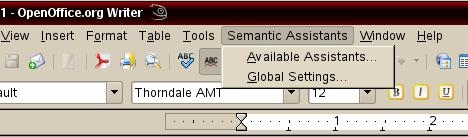
\includegraphics[width=0.7\textwidth]{pictures/oomenu.jpg}
\end{center}

In this menu, the user can inquire about available services, which are
selected based on the client (here \emph{Writer}) and the language
capabilities of the deployed NLP services (described in service
metadata, see Section~\ref{sec:owl}). The dynamically generated list
of available services is then presented to the user, together with a
brief description, in a separate window, as shown in
Figure~\ref{fig:oolist}. Note that the integration of a new service
does not require any changes on the client side---any new NLP service
created and deployed by a language engineer is dynamically discovered
through its OWL metadata maintained by the architecture and so becomes
immediately available to any connected client.
\begin{figure}[htb]
  \centering
  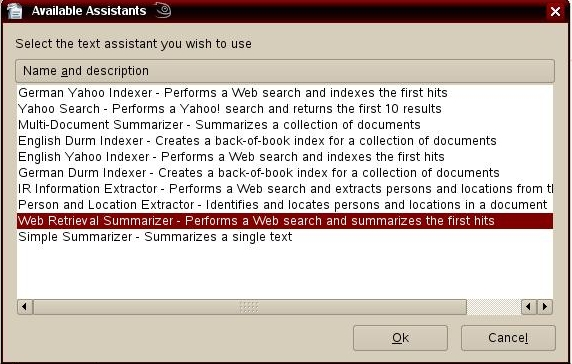
\includegraphics[width=0.5\textwidth]{pictures/oolist.jpg}
  \caption{List of available semantic assistants}
  \label{fig:oolist}
\end{figure}

The user can now select an assistant and execute it. In case the
service requires additional parameters, such as the length of a
summary to be generated, they are detected by our architecture through
the OWL-based service description and requested from the user through
an additional dialog window. An example, for the \emph{Web Retrieval
  Summarizer} assistant, is shown in Figure~\ref{fig:ooparams}.
\begin{figure}[htb]
  \centering
  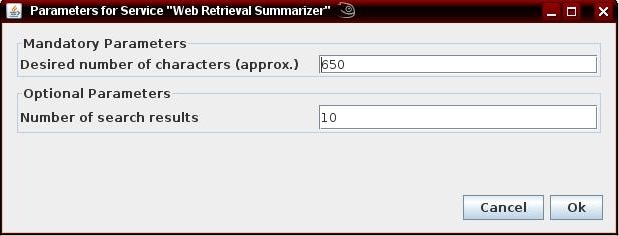
\includegraphics[width=0.5\textwidth]{pictures/ooparams.jpg}
  \caption{The parameters dialog, which appears when a Semantic
    Assistant requiring further input is invoked}
  \label{fig:ooparams}
\end{figure}
After the service is executed, the result is displayed in Writer depending on
the type of the server response: either as a new document, as annotations on
the existing document, or by opening an external viewer (e.g., a Web browser
for HTML documents).

\subsubsection{Side-Notes View}
The latest release of the OpenOffice.org Suite offer a new feature for text
annotation.  Depending on the annotation results received from GATE, the
Semantic Assistants Writer plug-in presents it in a sidenote manner (see
Figure~\ref{fig:sidenotes}).
\begin{figure}[htb]
  \centering
  %\vspace*{-9mm}
  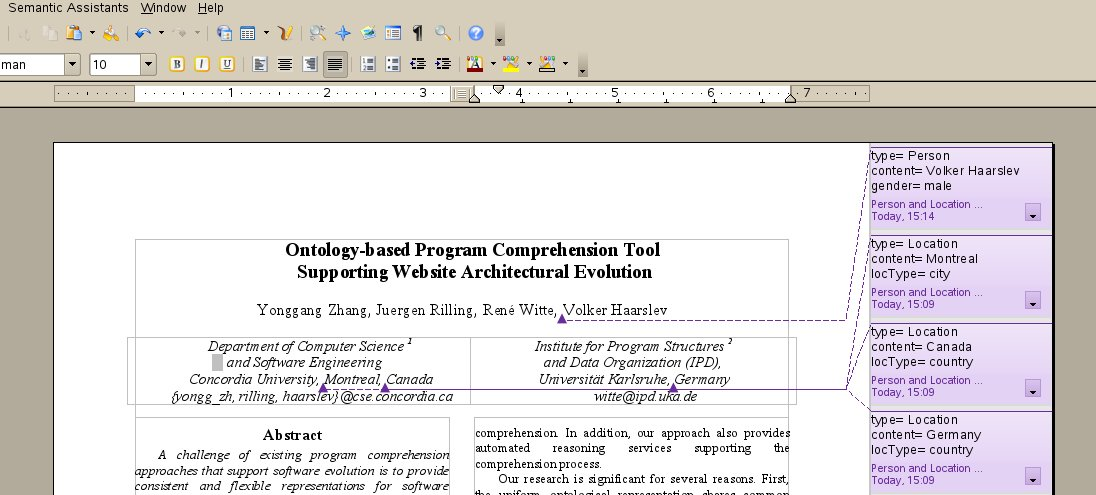
\includegraphics[width=0.8\textwidth]{pictures/sidenotes.jpg}
  \caption{Auto-Generated SideNotes Example}
  \label{fig:sidenotes}
  %\vspace*{-0.4cm}
\end{figure}

\subsubsection{New Document Creation}
\label{sec:doc-cre}
Creation of a new document comes handy when the output of an NLP service
corresponds to a complete document, or the result itself is indivisible. Some
examples are summarization or question-answering (see Figure~\ref{fig:oores}).

\begin{figure*}[htb]
  \centering
  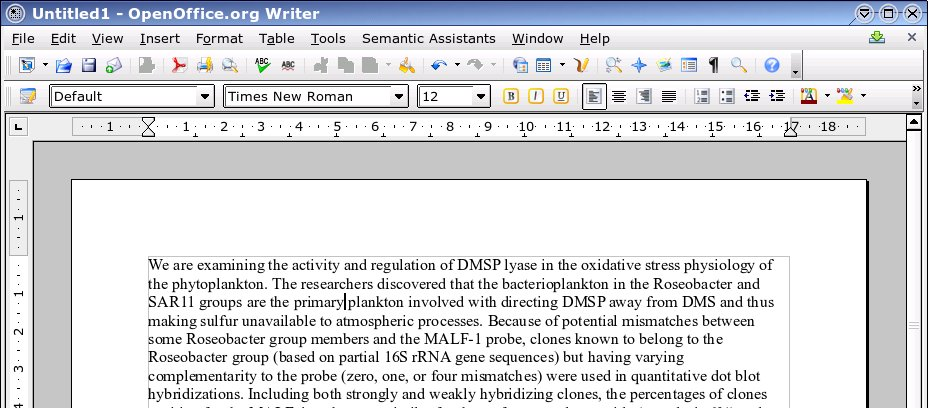
\includegraphics[width=0.8\textwidth]{pictures/ooresult_clip.jpg}
  \vspace*{-2mm}
  \caption{NLP services can also create a completely new document as a
  result (e.g., through summarization)}
  \label{fig:oores}
\end{figure*}

\subsubsection{Annotation Highlighting}
Besides text annotation, we offer the option for enabling/disabling annotation
highlighting for text that has been processed by GATE. This option can be
found under the Semantic Assistants menu in ``Global Settings.''  See
Figure~\ref{fig:highlight} for an example.

\subsubsection{Filter Empty Features}
This option found under the Semantic Assistants menu in ``Global Settings'' (shown
in Figure~\ref{fig:oosettings}) allows the ability to enable/disable filtering of
empty valued features in side-nodes. This can be useful to avoid cluttering or aid
debugging annotations respectively.

\subsubsection{Show Annotation Content}
This option in the ``Global Settings'' dialog can be used to include/exclude
the annotated content within the side-note. This can be used as an alternative
to annotation highlighting.

\begin{figure}
  \centering
  %\vspace*{-9mm}
  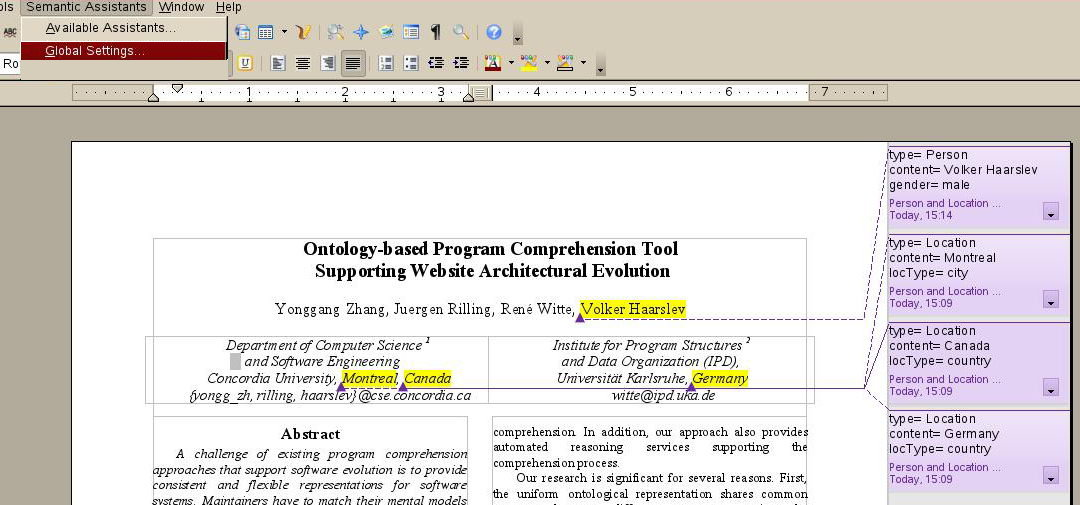
\includegraphics[width=0.8\textwidth]{pictures/highlighting.jpg}
  \caption{Highlighted Annotations Example}
  \label{fig:highlight}
  %\vspace*{0.5cm}
\end{figure}

\begin{figure}[htb]
\begin{center}
  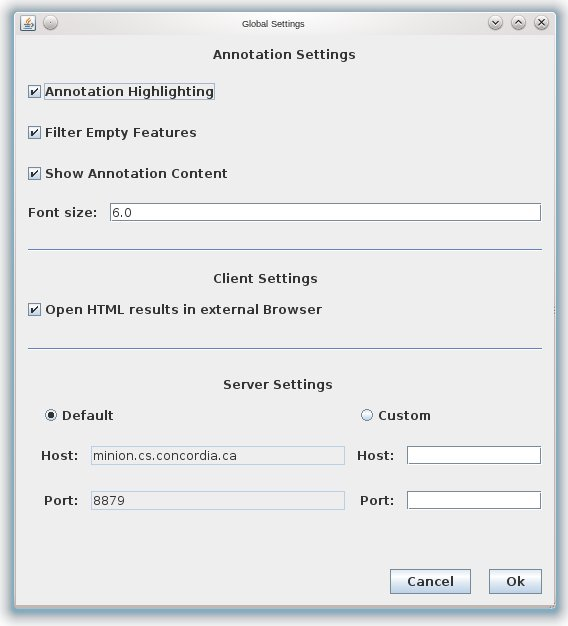
\includegraphics[width=0.5\textwidth]{pictures/oosettings.jpg}
  \caption{Configuration Dialog}
  \label{fig:oosettings}
\end{center}
\end{figure}

\subsubsection{Annotation Font Size}
As shown in Figure~\ref{fig:oosettings}, the font size of annotations can be changed
prior to invoking assistants. Due to the fixed width of side-notes, customizing the
size can ease readability of features.

\subsubsection{Browser Handling of HTML Results}
Instead of returning annotations, some pipelines produce HTML documents. The
"Open HTML results in external Browser" option shown in Figure~\ref{fig:oosettings},
allows OpenOffice to invoke a local browser to display these results.

\subsubsection{Server Settings}
Another option found under the Semantic Assistants menu in ``Global
Settings.''is \emph{Server Settings}.  There the user is able to specify the
Server information (Host and Port) of a local or distant server.

\subsection{Installation}
\label{subsec:oo-inst}
The OpenOffice.org plug-in can be found in
\url{SemanticAssistants/Clients/OpenOffice} and it is compatible with 
OpenOffice versions greater than 2.0.4. To use it, do the following:

\begin{enumerate}
  % TODO: what about the OO SDK installation? 
  % Is it needed for running the plug-in?

  \item Start OpenOffice.org Writer and ensure the right Java VM is
  used. Go to \emph{Tools $\rightarrow$ Options}. Under
  \emph{OpenOffice.org} you will find a \emph{Java} item. There, you
  can specify JREs. If it is not already there, add the currently used
  Java version.
  
  % should add screenshots for this
  \item Go to \emph{Tools $\rightarrow$ Extension Manager}. Click the
    \emph{Add$\ldots$} button on the bottom. Navigate to your local
    copy of the \sa\ architecture and then to
    \texttt{Clients/OpenOffice}. Select the file
    \texttt{SemassistOpenOfficePlugIn.oxt} and click \emph{Open}.

  \item Leave the dialog and open a new text document. You should have
    a new menu bar entry labeled \emph{Semantic Assistants}. Now you
    can run services on the current document (remember the server must
    be running to be able to query or execute language services).
\end{enumerate}


\subsection{Development Notes}
\label{sec:oo-spec}
In this section, we provide further technical details on our plug-in
for developers interesting in enhancing or modifying it.

\subsubsection{Compiling the Plug-in}
If you want to build the plugin yourself, follow these steps:
\begin{itemize}
  \item cd to the \url{Clients/OpenOffice} directory.

  \item Type \texttt{ant run}, or \texttt{ant run-gui}. Note that the
    client-side abstraction layer must have already been built and
    packaged. Both \texttt{ant run} and \texttt{ant run-gui} provide
    an UNO package named \url{SemassistOpenOfficePlugIn.oxt}. Both
    targets additionally copy it to \url{~/Documents/uno-components}.
    If \texttt{ant run-gui} is issued the OpenOffice.org
    \emph{Extension Manager} will pop up and prompt the user to
    install the extension.  If \texttt{ant run} is issued the above
    process is automated.  After the installation, OpenOffice Writer
    starts with the plug-in installed.

    \textbf{Note:} you can also manually add the plug-in from within
    OpenOffice (skip this step if you already used the \emph{run} or
    \emph{run-gui} target): Go to Tools, Extension Manager. Select
    \emph{My Extensions}, then click \emph{Add...} on the
    right. Choose the UNO package (available in
    \url{~/Documents/uno-components} if you used the \emph{deploy}
    target for ant).
\end{itemize}

\subsubsection{OpenOffice.org Plug-in Specifics}
Every plug-in has to include a \emph{description.xml} that describes the 
package's meta details like publisher, license, download url and version dependencies.
See \href{http://wiki.services.openoffice.org/wiki/Documentation/DevGuide/Extensions/Description_of_XML_Elements}{OpenOffice Developer's Guide}
for a list of available elements. The plug-in package also includes a
\emph{META-INF} directory, which contains a file called
\emph{manifest.xml}. This XML file lists the elements that come with
this plug-in;  The concrete manifest file for our plug-in is listed in
Figure~\ref{list:manifest}.  We can see that it defines three
\emph{file-entry} elements specifying the type and location of the
following files:
\begin{figure}[tb]
\centering
\begin{lstlisting}[language=XML,numbers=left,xleftmargin=8mm,columns=flexible]
<?xml version="1.0" encoding="UTF-8"?> 
<!DOCTYPE manifest:manifest PUBLIC 
"-//OpenOffice.org//DTD Manifest 1.0//EN" "Manifest.dtd"> 
<manifest:manifest 
 xmlns:manifest="http://openoffice.org/2001/manifest"> 
  <manifest:file-entry 
     manifest:media-type=
        "application/vnd.sun.star.configuration-data" 
     manifest:full-path="Addons.xcu"/> 
  <manifest:file-entry 
     manifest:media-type=
        "application/vnd.sun.star.configuration-data" 
     manifest:full-path="ProtocolHandler.xcu"/> 
  <manifest:file-entry 
     manifest:media-type=
        "application/vnd.sun.star.uno-component;type=Java" 
     manifest:full-path=
        "ProtocolHandlerAddon_java.uno.jar"/>
   <!-- Add any other plug-in required jar files here. -->
</manifest:manifest> 
\end{lstlisting}
\caption{The \emph{manifest.xml} file for our plug-in}
\label{list:manifest}
\end{figure}


\begin{description}
\item[\emph{Addons.xcu}.] This XML file defines how the plug-in should
  be integrated with OpenOffice.org. In our case, it contains a menu
  definition, specifying that the menu should only appear in the
  \emph{Writer} application. For each menu item, we specify which
  messages should be broadcast throughout the OpenOffice.org runtime
  system when the menu item is activated.
\item[\emph{ProtocolHandler.xcu}. ] This XML file specifies that the
  messages defined in \emph{Addons.xcu} should be handled by an object
  of a certain class. This class is provided in the Java archive and
  must adhere to a certain interface. 
\item[\emph{ProtocolHandlerAddon\_ java.uno.jar}.] This Java archive
  contains the actual functionality of the plug-in. It holds classes
  responsible for receiving the messages generated by the menu items,
  as well as classes responsible for the interaction with the
  client-side abstraction layer.
\end{description}


\subsubsection{Implementation Details}
A useful class called \url{UNOUtils} found in the \url{package
  info.semanticsoftware.semassist.client.openoffice.utils} contains most of
the OO-Writer feature implementations.  More specifically, the three methods in
Figure~\ref{list:ssb} implement a major part of the above described features
(Side-Notes, Highlighting and New Document Creation).

\begin{figure}
\centering
\begin{lstlisting}[language=Java,numbers=left,xleftmargin=8mm,columns=flexible]

private static XComponent CreateNewDocument( XDesktop xDesktop, 
					     String sDocumentType )
{
	...
}

private static void AnnotateField( Annotation annotation )
{
	...
	// Use the text document's factory to create an Annotation text field
	XTextField xAnnotation = (XTextField) UnoRuntime.queryInterface(
		XTextField.class, mxDocFactory.createInstance(
		"com.sun.star.text.TextField.Annotation" ) );
	
	// get the properties of the field
	XPropertySet xPropertySet = (XPropertySet) UnoRuntime.queryInterface( 
						XPropertySet.class, xAnnotation
);
	
	...
	
	// Highlight annotated field
        HighlightField();
}

private static void HighlightField()
{
....

}
\end{lstlisting}
\caption{Core methods implementing the OpenOffice Writer plug-in features are
  part of the \texttt{UNOUtils} class}
\label{list:ssb}
\end{figure}

%More details on how to compile and debug an OpenOffice plug-in can be found in Section~\ref{sec:debug}.
 
\subsubsection{Configure the OpenOffice Writer to Run in Debug Mode}
This Section describes how to configure the JAVA VM in OpenOffice Writer to accept incoming connection for a debugger.

\begin{enumerate}
  \item Open OpenOffice Writer
  \item Go to Tools, Options. Under \emph{OpenOffice.org}, there is a \emph{Java} item. Select it and then Click on the 
        \emph{Parameter} button. There the parameters when running the JAVA VM are set.
  \item To run in debug mode \emph{Assign} the following 2 parameters:
  \begin{itemize}
    \item \textbf{-X debug}
    \item \textbf{-Xrunjdwp:transport=dt\_socket,server=y,suspend=n,address=7081}
  \end{itemize}
  \item \textbf{Note: The} \emph{address=7081} \textbf{should be the consistent with the port set within the debugger}
  \item  Now OO Writer is ready to accept connections from the debugger
\end{enumerate} 


\section{Eclipse Plug-in}
Eclipse is not a single monolithic program, but rather a small kernel containing
a plug-in loader surrounded by hundreds of plug-ins. The behavior of each
plug-in in this architecture is stored in its code, and its dependencies and
services are declared in the plug-in's manifest file. On each Eclipse startup,
the plug-in loader scans all the available manifest files in the Eclipse
exclusive plug-in folder and then builds a structure containing this
information.

We used this characteristic of Eclipse architecture to integrate our Semantic
Assistants architecture into the Eclipse environment in form of a plug-in, in
order to offer various Natural Language Processing services. The Semantic
Assistants Eclipse plug-in is basically a Java archive (JAR) file that ships
with its own specific content and a description file to introduce itself to the
Eclipse plug-in loader. 

\subsection{Features}
Once the Semantic Assistants plug-in is installed, it creates a new menu entry
in the Eclipse menu toolbar. A user can inquire about the available services
from the "Available Assistants" item and modify the connection settings to the
Semantic Assistants server by selecting the second item.
\begin{figure}[htb]
\begin{center}
  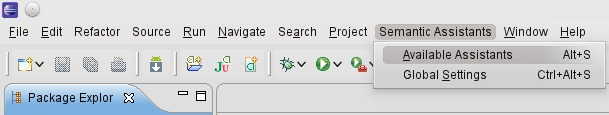
\includegraphics[width=1.0\textwidth]{pictures/eclipse_menu.jpg}
  \caption{Semantic Assistant Menu in Eclipse}
  \label{fig:eclipse_menu}
\end{center}
\end{figure}
\subsubsection{Available Assistants}
Selecting the "Available Assistants" item from Semantic Assistants menu will
open a file selection dialog. The file selection dialog allows the user to
select the desired files, folders and even complete projects to send to the
server as inputs to an NLP service. For more convenience, you can type an arbitrary extension like ``java'' or ``xml'', in the ``File Format'' field to filter to file tree view. 

\begin{figure}[htb]
\begin{center}
  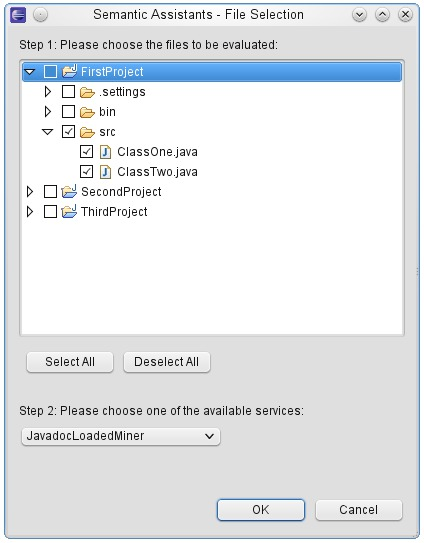
\includegraphics[width=0.5\textwidth]{pictures/eclipse_fileSelection.jpg}
  \caption{File Selection Dialog}
  \label{fig:eclipse_fileSelection}
\end{center}
\end{figure}

This dialog also lets the user to select an NLP service from a dynamically
generated list of services. This list is generated dynamically by selecting the
available services based on the client and the language capabilities of the
deployed NLP services. The server location where the service information are read from is presented just above the list as depicted in Fig \ref{fig:eclipse_services}. Note that the integration of a new service does not
require any changes on the client side - any new NLP service created and
deployed by a language engineer is dynamically discovered through its OWL
metadata maintained by the architecture and so becomes immediately available to
any connected client.

\begin{figure}[htb]
\label{fig:eclipse_services}
\begin{center}
  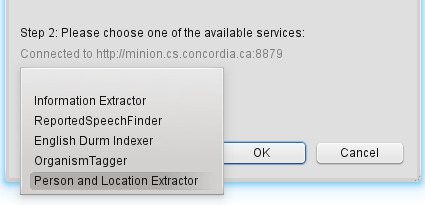
\includegraphics[width=0.5\textwidth]{pictures/eclipse_services.jpg}
  \caption{A List of Available NLP Services}
  \label{fig:eclipse_services}
\end{center}
\end{figure}

Upon selecting the resource files and the desired service, the user can execute
the selected service on the checked files in the tree. Consequently, the user will be informed about the status of the execution in the ``Semantic Assistant Status'' view. A successful execution of the selected NLP service, will let the user know on how to view the results. If the service execution fails, a description of the occurred error will be shown to the user and invocation will be aborted.

Now, let's look at how different types of outputs are handled in the plug-in:

\paragraph{Annotations.}
Annotations retrieved from a successful service invocation are being shown to the user in an
Eclipse view part called "Semantic Assistants" view. In the mentioned view, a
table will be dynamically generated that contains
all the parsed annotation instances. In Figure~\ref{fig:eclipse_saView} the
result of an execution of the "Person and Location Extractor" service on two
sample classes is shown.
\begin{figure}[htb]
\begin{center}
  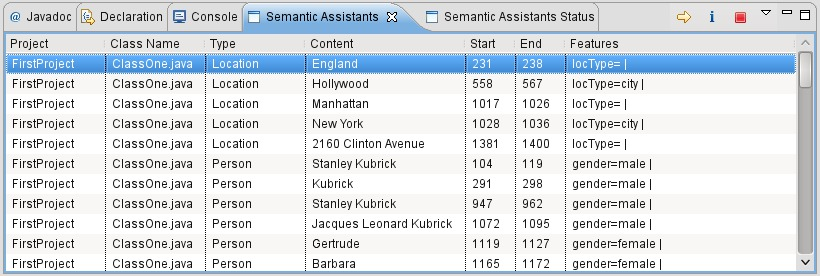
\includegraphics[width=1\textwidth]{pictures/eclipse_saView.jpg}
  \caption{Semantic Assistants View}
  \label{fig:eclipse_saView}
\end{center}
\end{figure}

This table can be sorted by different criteria through clicking on each column
title. Additionally, by double-clicking on each row in the table, the selected
annotation will appear with a graphical representation attached to the
corresponding resource. For instance, in Figure~\ref{fig:eclipse_annotation} the
JavadocMiner service has been invoked on a Java source code file. Some of the
annotations returned by the server bear a \emph{lineNumber} feature, which
attaches an annotation instance to a specific line in the java source file. Upon
double-clicking on the annotation instance in the Semantic Assistant view, the
corresponding resource - here, a .java file - will be opened in an editor and an
Eclipse warning marker will appear next to the line defined by the annotation
\emph{lineNumber} feature.

\begin{figure}[htb]
\begin{center}
  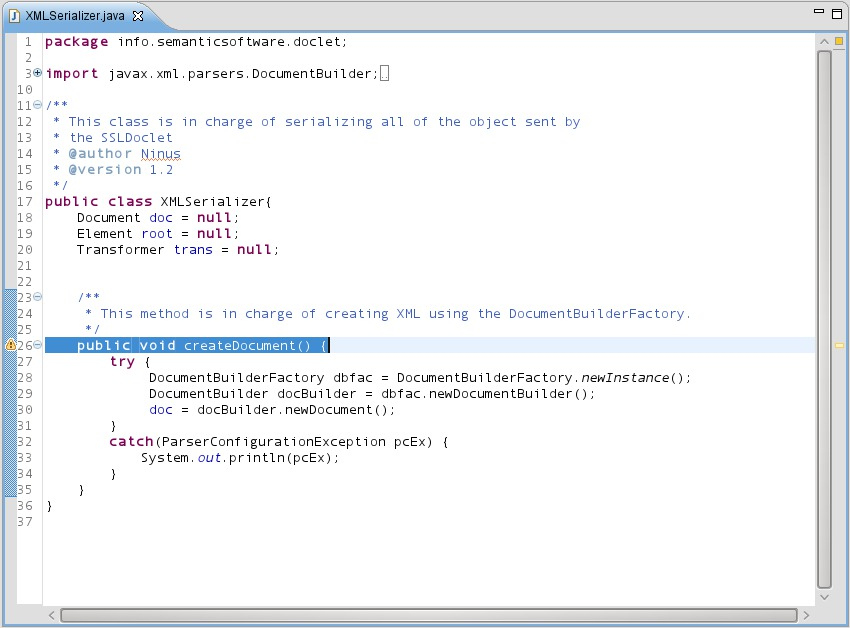
\includegraphics[width=1\textwidth]{pictures/eclipse_annotation.jpg}
  \caption{A Semantic Annotation}
  \label{fig:eclipse_annotation}
\end{center}
\end{figure}

\paragraph{Boundless Annotations.}
Boundless Annotations are a special kind of Annotations that adhere to a whole document and thus have no start and end offset. The plug-in parses the annotation results, and then inserts the content of the annotations in a new document and opens it in a new editor inside the Eclipse environment.

\paragraph{Documents.}
Documents received from the server response carry a URL property where defines where they are located. The plug-in retrieves the URLs and inserts them into a new document that opens up in a new editor inside the Eclipse environment.

\paragraph{Files.}
When a file output type is received by the plug-in, it will try to open it up in a web browser. In Eclipse, users can configure whether they want to open URLs in the Eclipse built-in web browser or any other ones in the file system. Whichever defined as the default behavior in Eclipse by the user, will be used by the plug-in to present the result file to the user. In this case, a log message will be shown to the user in the ``Semantic Assistants Status'' view to inform the user that the file is opened in his browser.

\subsubsection{Global Settings}
The second option found under the Semantic Assistants menu is the "Global
Settings" item. By clicking on this menu item, a dialog as depicted in Figure \ref{fig:eclipse_settings} is shown to the user that lets him choose a preferred server from a list of pre-defined values or add a custom server to the settings file. The values are provided in the Semantic Assistants global preference file described in \ref{sec:pref_management}. If the preference file gets accidentally deleted, a default preference file will be created by the plug-in but the eclipse-specific settings will be lost.
\begin{figure}[htb]
\begin{center}
  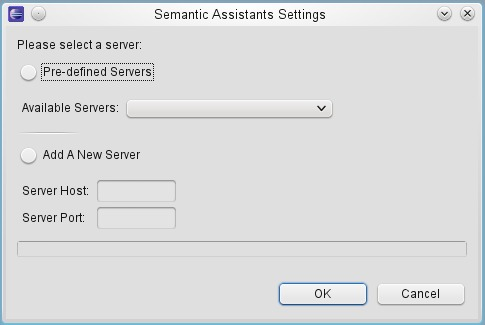
\includegraphics[width=0.6\textwidth]{pictures/eclipse_settings.jpg}
  \caption{Semantic Assistants Server Settings Dialog}
  \label{fig:eclipse_settings}
\end{center}
\end{figure}

\subsection{Installation}
\label{subsec:eclipse_install}
You can install the Semantic Assistants plug-in via the Eclipse software installer. To do so, first you have to add the Semantic Assistants software repository to your Eclipse list of software sites. In addition to installing the plug-in, adding the repository lets the Eclipse update manager to check for plug-in updates once available. Please carefully follow the steps listed below to install the Eclipse plug-in and refer to section \ref{trouble:eclipse_install} for installation troubleshooting.

\begin{enumerate}
  \item Select Help $\rightarrow$ Install New Software to open the Eclipse software installer.
  \item Press the ``Add'' button in the dialog, to add the Semantic Assistants repository.
  \item In the new dialog depicted in Fig \ref{fig:eclipse_install}, type ``\texttt{Semantic Assistants}'' and\\ ``\texttt{http://sa-eclipse.semanticsoftware.info}'' in ``Name'' and ``Location'' fields, respectively, and press ``OK''.
  \item The Semantic Assistants repository should now be added to your Eclipse list of software sites as seen in Fig \ref{fig:eclipse_install2}. From the loaded softwares, check the Eclipse plug-in and press ``Next''.
  \item Simply, follow the installation steps and let the installer restart the Eclipse application.
  \item The Eclipse plug-in loader will automatically load the plug-in for you. If the plug-in is installed
successfully, you should be able to see the Semantic Assistants menu added to
you toolbar.
\end{enumerate}

\begin{figure}[htb]
\begin{center}
  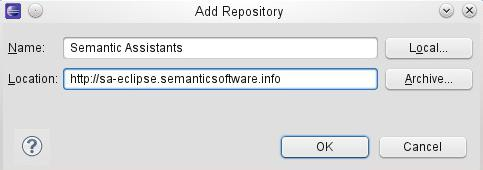
\includegraphics[width=0.6\textwidth]{pictures/eclipse_install.jpg}
  \caption{Adding Semantic Assistants Repository to Eclipse List of Software Sites}
  \label{fig:eclipse_install}
\end{center}
\end{figure}

\begin{figure}[htb]
\begin{center}
  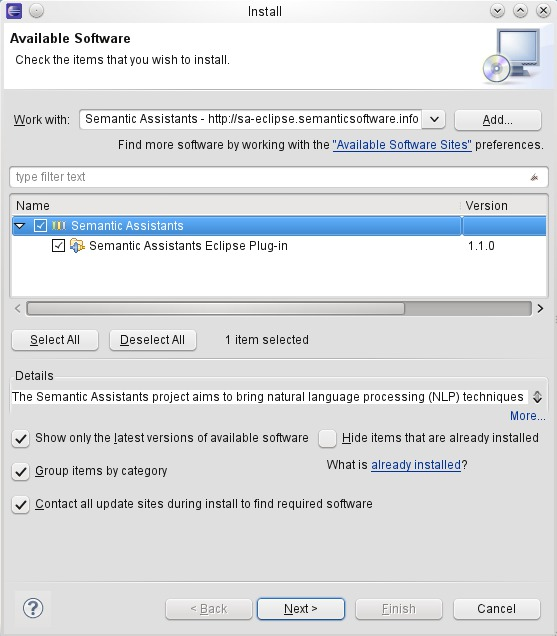
\includegraphics[width=0.6\textwidth]{pictures/eclipse_install2.jpg}
  \caption{Eclipse Software Installer Dialog}
  \label{fig:eclipse_install2}
\end{center}
\end{figure}

\subsection{Updating The Plug-in}
\begin{enumerate}
  \item Select Help $\rightarrow$ Check for Updates to open the Eclipse update manager.
  \item If there are any updates available for the Semantic Assistants plug-in, it will appear the in the update manager dialog as shown in Fig \ref{fig:eclipse_update}.
  \item Check the Semantic Assistants Eclipse plug-in from the list and press ``Next''.
  \item Follow the wizard steps and let the update manager restart your Eclipse for the updates to take place.
\end{enumerate}

\begin{figure}[htb]
\begin{center}
  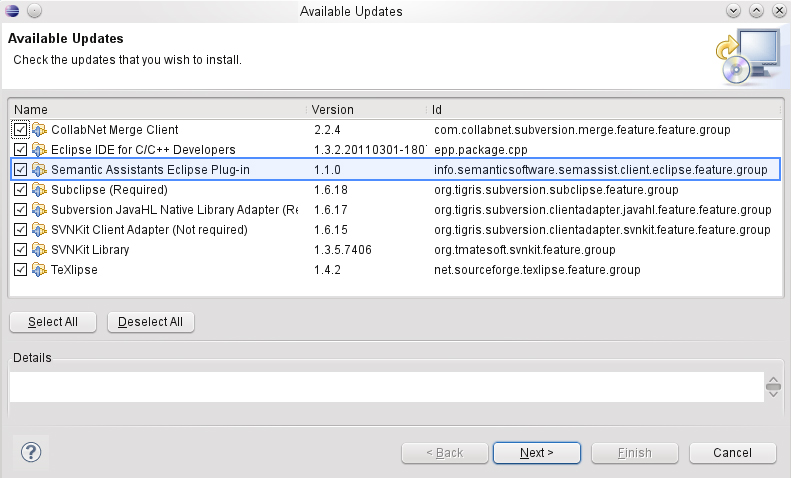
\includegraphics[width=1.0\textwidth]{pictures/eclipse_update.jpg}
  \caption{Updatin the Plug-in via Eclipse Update Manager}
  \label{fig:eclipse_update}
\end{center}
\end{figure}

\subsection{Development Notes}
\label{subsec:eclipse.development}
In this section, we provide further technical details on our plug-in for
developers interesting in enhancing or modifying it.

\subsubsection{Plug-in Source Directory Structure}
The Semantic Assistants plug-in uses Model-View-Controller pattern for its
implementation. Thus, most of the source code files are divided into different
packages related to their responsibilities. When you browse to
\url{src/info/semanticsoftware/semassist/client/eclipse/} folder, you see the
following structure:
\begin{enumerate}
\item\url{dialogs}: This folder contains the dialogs that are shown to the user
for interactions e.g. file selection. The classes inside this folder are the
codes for graphical user interfaces.
\item\url{handlers}: This folder contains the classes which play the controller
role in MVC pattern. Examples of these classes are dialog handlers and service
invocation jobs.
\item\url{model}: This folder contains the classes that provide data for
graphical user interfaces. These models are consumed by classes inside
\texttt{views} package.
\item\url{utils}: This folder contains utility classes e.g. logging feature.
\item\url{views}: This folder contains the source codes for Semantic Assistants
view parts. These are again graphical user interfaces but packaged differently
from dialogs.
\end{enumerate}

There is also another file called \url{Activator.java} in the source directory.
It is the main class of the plug-in that will be loaded initially and control
the plug-in's life cycle.

\subsubsection{Modifying the Plug-in}
If you want to modify the plug-in behavior or enhance it, follow these steps:
\begin{enumerate}
\item Open the Eclipse application.
\item Select File $\rightarrow$ New  $\rightarrow$ Project and under the
"Plug-in Development" category select the "Plug-in Project".
\item A new plug-in project wizard will open up. Keep the EclipsePlugin name for
the project. Just below the project name there is a checkbox reading "Use
Default Location". Uncheck it and browse to the EclipsePlugin folder inside
where you've stored the Semantic Assistants folder.
\item Leave the other options untouched and press Finish.
\end{enumerate}

\begin{figure}[htb]
\begin{center}
  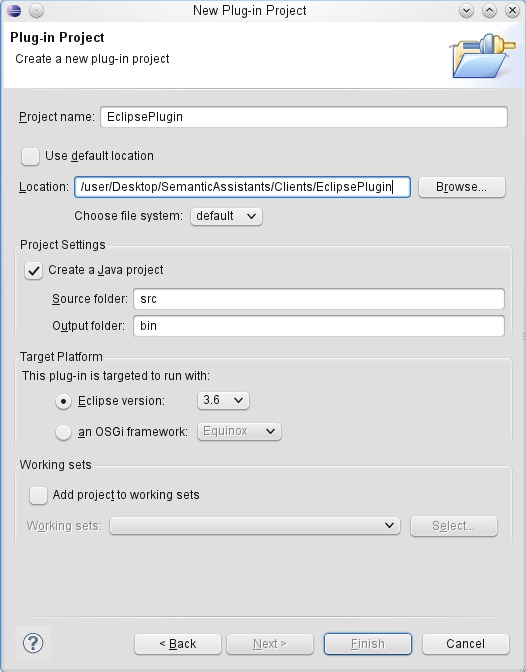
\includegraphics[width=0.5\textwidth]{pictures/eclipse_project_wizard.jpg}
  \caption{Eclipse New Plug-in Project Wizard}
  \label{fig:eclipse_project_wizard}
\end{center}
\end{figure}

\textbf{Note:} Remember you should manually copy the CSAL.jar file into you the
project's \texttt{lib} folder because it is a part of the project's dependency
and is defined in the classpath.

When the project is loaded in your workspace, feel free to play around. Browse
the source directory and add your development codes. To run your code, right
click on \texttt{plugin.xml} file and select Run As $\rightarrow$ Eclipse
Application.

\section{Global Preference Management}
\label{sec:pref_management}
Semantic Assistants clients preferences are stored in a single file in the user machine's home directory under the name \texttt{semassist-settings.xml}. This file is shared between all the clients and contains information, such as different servers that clients can connect to as well as other client-specific preferences. The preference XML document has two main parts: a global part and a client-specific part. The scope of the global preference, as the name suggests, is all of the clients and any changes to this part will affect them all. The client-specific scope, on the other hand, is limited to that specific client and does not affect others. Each Semantic Assistants client installed on the user machine has a dedicated tag inside the client-specific part, where it can store its proprietary preferences.

This file does not ship with the Semantic Assistants project but a default preference file is created by the very first client installed and used on the user's machine and will be reused by the subsequent clients. It is not advised to manually modify this file unless its structure can be kept consistent. In case of deletion, a default file will be again created by the next used client. The structure of the preference file is detailed in \ref{client_pref}.